
\documentclass[a4paper]{report}
\documentclass[14pt]{extarticle} %Класс позволяет использовать базовые шрифты бОльших размеров
\usepackage[utf8x]{inputenc} %кодировка файла макета utf8
\usepackage[russian]{babel} 
\usepackage[left=25mm,right=15mm,top=12mm,bottom=20mm]{geometry} %Попытка разобраться с полями страниц
\usepackage{ntheorem} %окружение для настройки теорем 
\usepackage{graphicx} %работа с рисунками
\usepackage[labelsep=period,figurewithin=none,tablewithin=none]{caption} %подписи к объектам (рисунки, таблицы)
\usepackage{listings} %работа с листингами
\usepackage{indentfirst} %отступ первого абзаца в разделе
\usepackage{enumitem} %настройка маркированных и нумерованных списков (см. примеры настройки в тексте)
\usepackage{url} %формирование ссылок на электронные источники
\usepackage{fancyhdr} %Настройка нумерации страниц
\usepackage{tocloft} %Настройка заголовка для содержания

% \usepackage[T1]{fontenc}
% \usepackage[utf8]{inputenc}
% \usepackage{amsmath,amssymb}
% \usepackage[russian]{babel}

\usepackage{geometry} % Меняем поля страницы
\geometry{left=2cm}% левое поле
\geometry{right=2cm}% правое поле
\geometry{top=1.25cm}% верхнее поле
\geometry{bottom=1.5cm}% нижнее поле
\usepackage{indentfirst}

\begin{document}
\chapter*{Архитектура веб-сервиса Twitch.tv}

\section*{Требования к качеству}
\subsection*{Тип приложения}
Веб-приложение для выполнения преимущественно на сервере в сценариях с постоянным подключением.
\subsection*{Ключевые характеристики качества}
\begin{table}[h!]
  \centering
  \caption{}
  \label{t1}
  \begin{tabular}{|c|c|}
    \cline{1-2}
    Внешние характеристики ПО: Оценка  &Внутренние характеристики ПО:    Оценка\\ \cline{1-2}
    Корректность             6  & Удобство сопровождения               10\\ \cline{1-2}
    Практичность             10 & Гибкость                             8\\ \cline{1-2}
    Эффективность            9  & Портируемость                        8\\ \cline{1-2}
    Надежность               6  & Возможность повторного \tabularnewline & использования 5\\ \cline{1-2}
    Целостность              6  & Удобочитаемость                      6\\ \cline{1-2}
    Адаптируемость           8  & Тестируемость                        6\\ \cline{1-2}
    Правильность             6  & Понятность                           6\\ \cline{1-2}
    Живучесть                8  &  \\
    \cline{1-2}
  \end{tabular}
\end{table}
На основе таблицы выделим три наиболее значимых характеристики и сконцентрируемся на них. Таковыми являются: практичность, эффективность, удобство сопровождения. Практичность важна, потому что сервис нацелен на широкую аудиторию и тут необходима простота взаимодействия с сервисом. Эффективность важна, так же из-за обширности целевой аудитории, потому, что скорость работы сервиса очевидно прямо влияет на его успех у конечного пользователя. Удобство сопровождение важно потому, что широкая аудитория предполагает быструю масштабируемость и её не достичь без легкого изменения программной системы. Как следствие важности удобства сопровождения следует важность гибкости системы. Для данного приложения важно так же адаптируемость, потому что предполагается использование сервиса в том числе и на мобильных устройствах и как следствие этого во внутренних характеристиках системы становится важной портируемость системы. И наконец, из-за потенциально широкой аудитории и большого траффика (напомню, что Twitch.tv - сервис видеотрансляций) необходимо обеспечить высокую живучесть системы.

\section*{Координационная модель}
\subsection*{Стиль архитектуры}
Трехуровневая архитектура (клиент - сервер - сервер БД)
\subsection*{Ключевые требования к функциональности системы}
Основная функциональность системы в предоставлении возможности запустить свою видеотрансляцию через стороннее клиентское ПО и поместить ссылку на данную трансляцию в каталог сервиса. Нужно учитывать большую аудиторию и потому отдавать видео поток не напрямую с машины клиента, а кэшируя на сервере и отдавая конечному пользователю с минимальной задержкой.

\subsection*{Функциональные требования к системе в формате User Story}
A - авторизованный пользователь

N - неавторизованный пользователь
\begin{table}[h]
  \centering
  \label{t5}
  \footnotesize
  \begin{tabular}{|l|c|l|l|}
    \cline{1-4}
    \begin{tabular}[c]{@{}l@{}}Просмотр каталога трансляций\\ сгруппированные по играм\end{tabular}
 & N & 
       \begin{tabular}[c]{@{}l@{}}Нажатие на кнопку "Каталог"\end{tabular} & \begin{tabular}[c]{@{}l@{}}Появление страницы со списком \\трансляций и информации о них\end{tabular} \\ \cline{1-4}
    \begin{tabular}[c]{@{}l@{}}Просмотр трансляции\end{tabular}
 & N & 
       \begin{tabular}[c]{@{}l@{}}Нажатие на элемент каталога \\ трансляций\end{tabular} & \begin{tabular}[c]{@{}l@{}}Открытие страницы с трансляцией\end{tabular} \\ \cline{1-4}
    \begin{tabular}[c]{@{}l@{}}Комментирование трансляции\end{tabular}
 & A & 
       \begin{tabular}[c]{@{}l@{}}Ввод сообщения и нажатие\\на кнопку "Отправить"\end{tabular} & \begin{tabular}[c]{@{}l@{}}Появление сообщения пользователя\\в блоке комментариев\end{tabular} \\ \cline{1-4}
    \begin{tabular}[c]{@{}l@{}}Создание собственной трансляции\end{tabular}
 & A & 
       \begin{tabular}[c]{@{}l@{}}Заполнение формы создания трансляции\\и нажатие на кнопку "Создать"\end{tabular} & \begin{tabular}[c]{@{}l@{}}Появление трансляции в каталоге\\ сервиса\end{tabular} \\ \cline{1-4}
    \cline{1-4}
  \end{tabular}
  \normalsize
\end{table}
\subsection*{USE-CASE диаграмма}
\begin{figure}[h]
  \centering
  % Рамка только для изображений с белым фоном
  \fbox{
\includegraphics[scale=0.35]{img/use-case.png}}
  \caption{}
  \label{third}
\end{figure}

\subsection*{Основные программные модули системы}
\begin{enumerate}
\item Модуль регистрации/аутентификации/авторизации (сквозная функциональность)
\item Модуль создания трансляции
\item Модуль просмотра трансляции
\end{enumerate}
\begin{figure}[h!]
  \centering
  % Рамка только для изображений с белым фоном
  \fbox{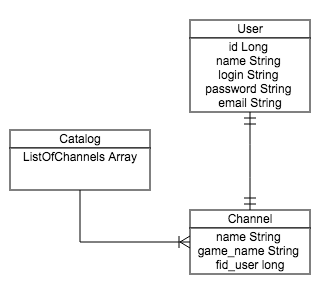
\includegraphics[scale=0.7]{img/er.png}}
  \label{third}
\end{figure}

\section*{Управление ресурсами}
\subsection*{Тип хранения данных}
СУБД
\subsection*{Реляционнная СУБД}
Реляционная СУБД: Postgresql. Уровень изоляции: read committed. SQL.

Выбор Postgresql был основан на сравнении с MySQl. У СУБД MySQL есть очень хорошее преимущество для высоконагруженных проектов, это механизм репликации. Репликация — одна из техник масштабирования баз данных. Состоит в том, что данные с одного сервера базы данных постоянно копируются (реплицируются) на один или несколько других (называемые репликами). Для приложения появляется возможность использовать не один сервер для обработки всех запросов, а несколько. Таким образом  можно распределить нагрузку с одного сервера на несколько. Но MySQL использует механизм подключаемых search engines (например InnoDB и MyISAM) и из-за этого репликация реализуется неэффективным способом.
\subsection*{Связи между элементами архитектуры}
\begin{figure}[h!]
  \centering
  % Рамка только для изображений с белым фоном
  \fbox{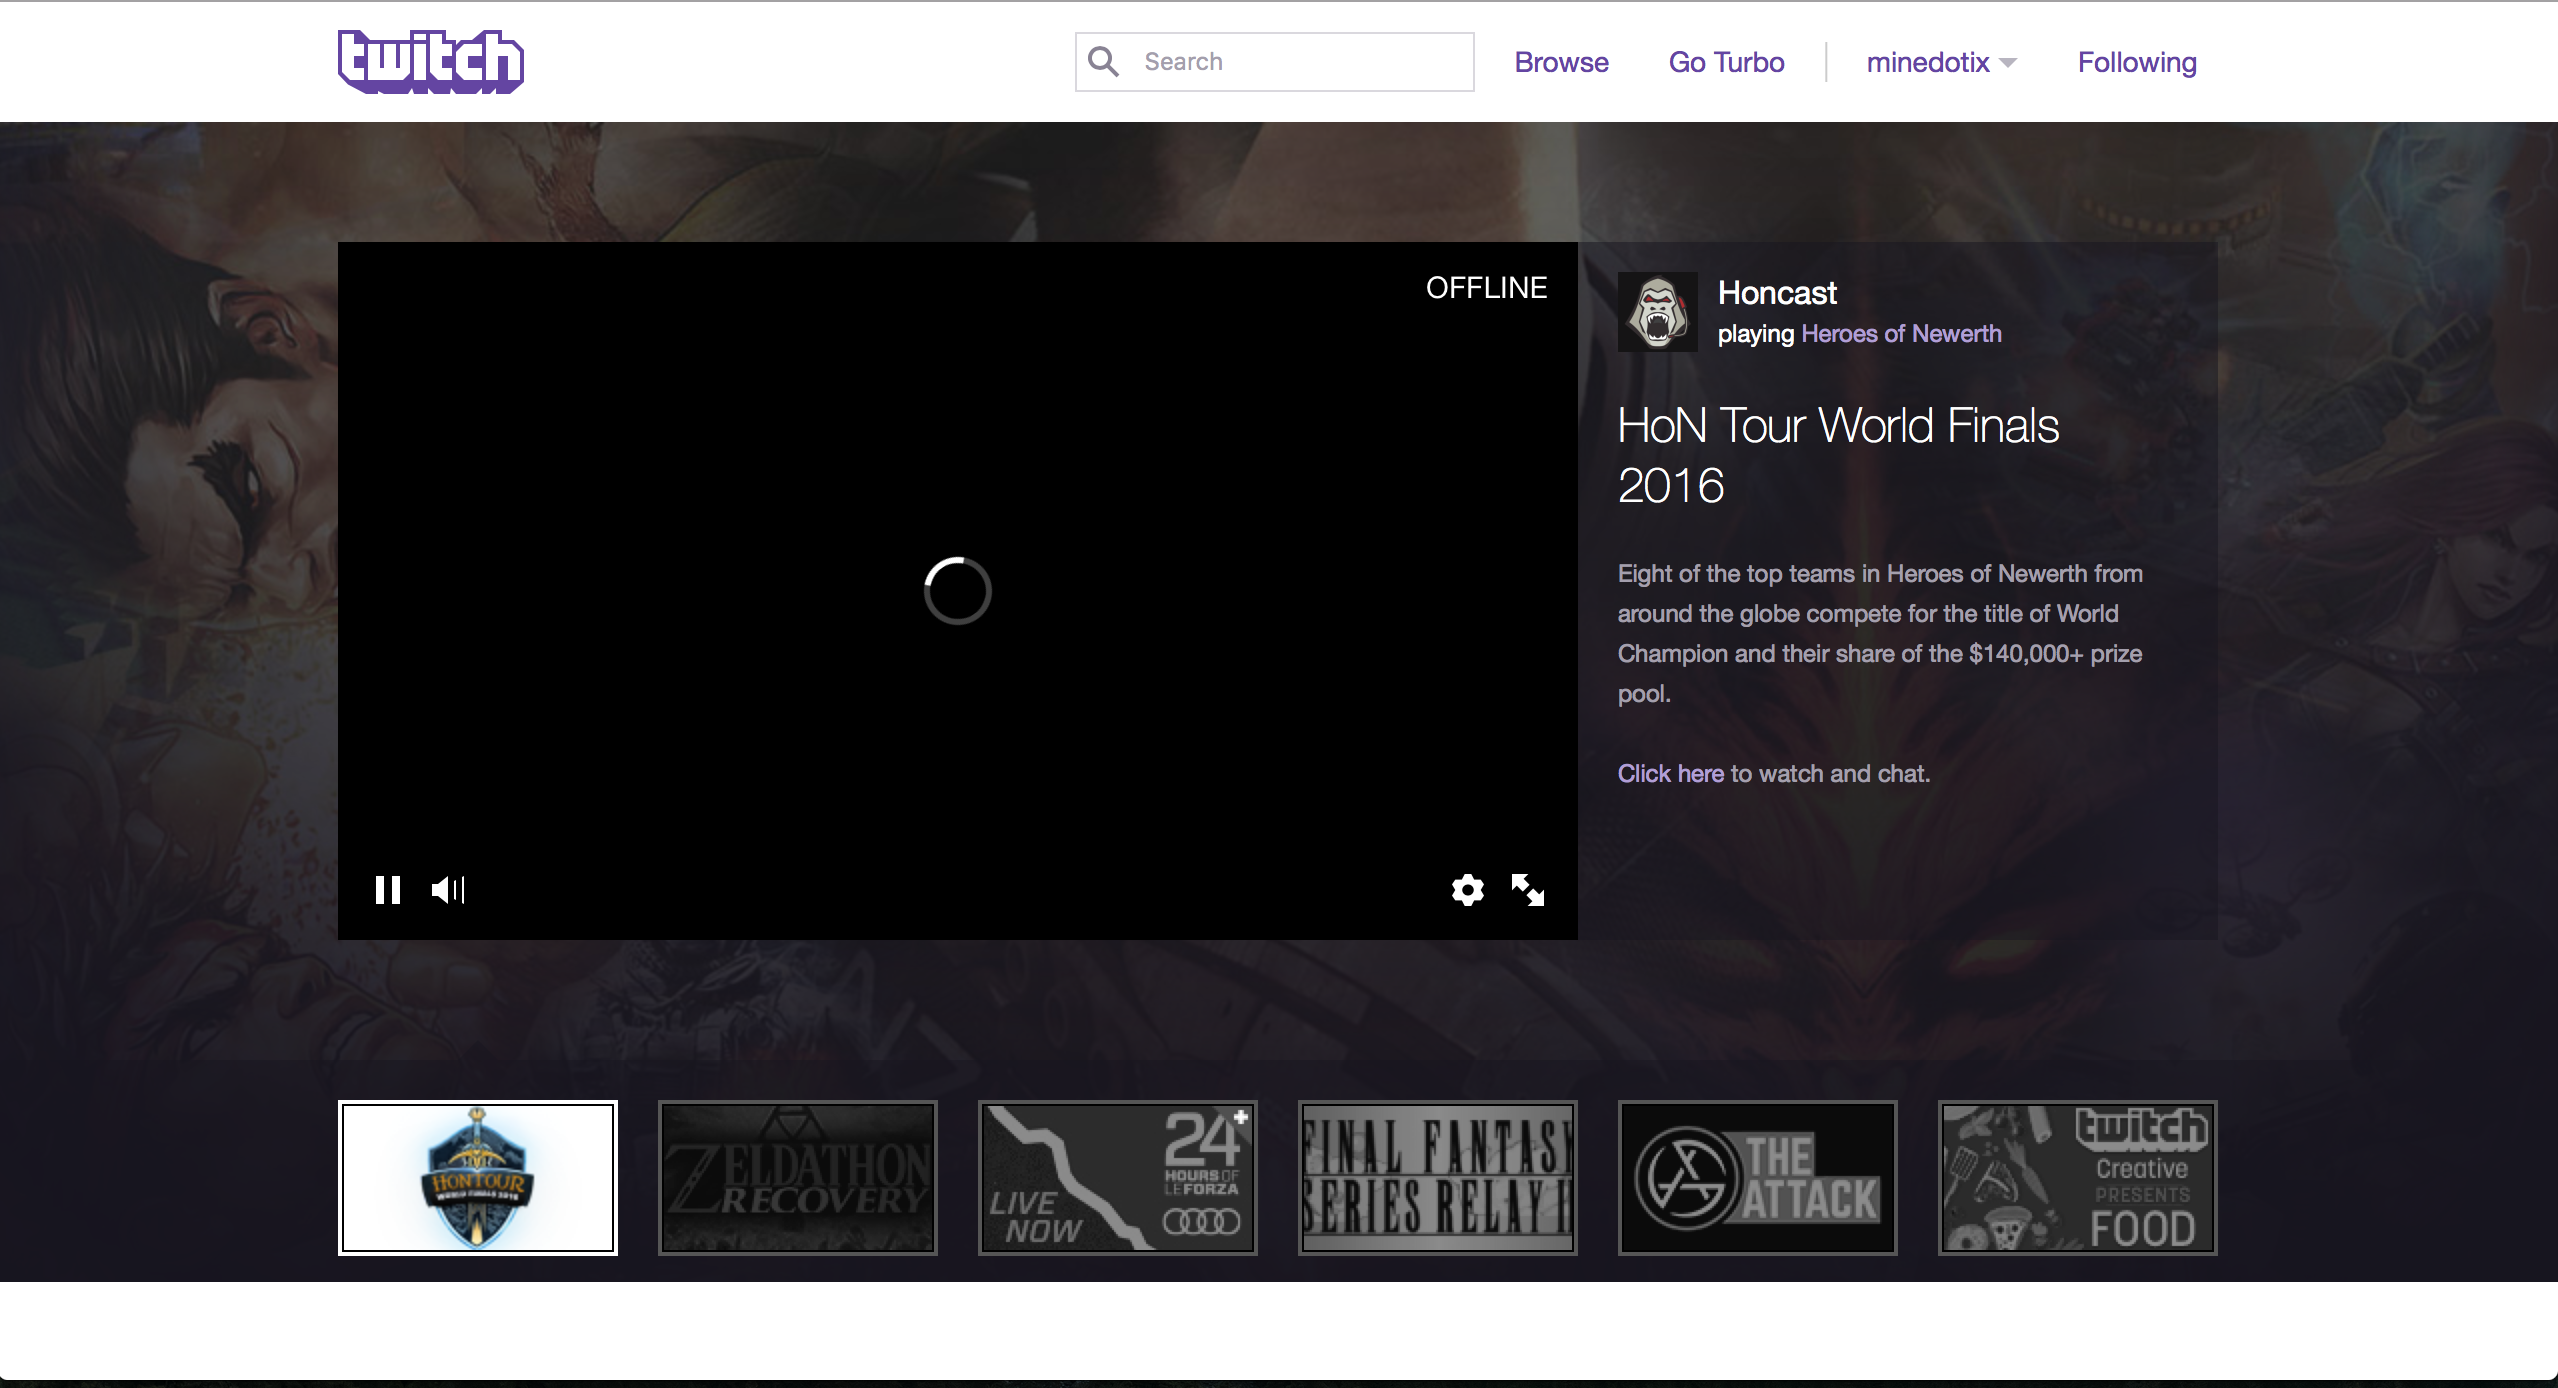
\includegraphics[scale=0.3]{img/main.png}}
  \caption{Главная страница}
  \label{third}
\end{figure}

\begin{figure}[h!]
  \centering
  % Рамка только для изображений с белым фоном
  \fbox{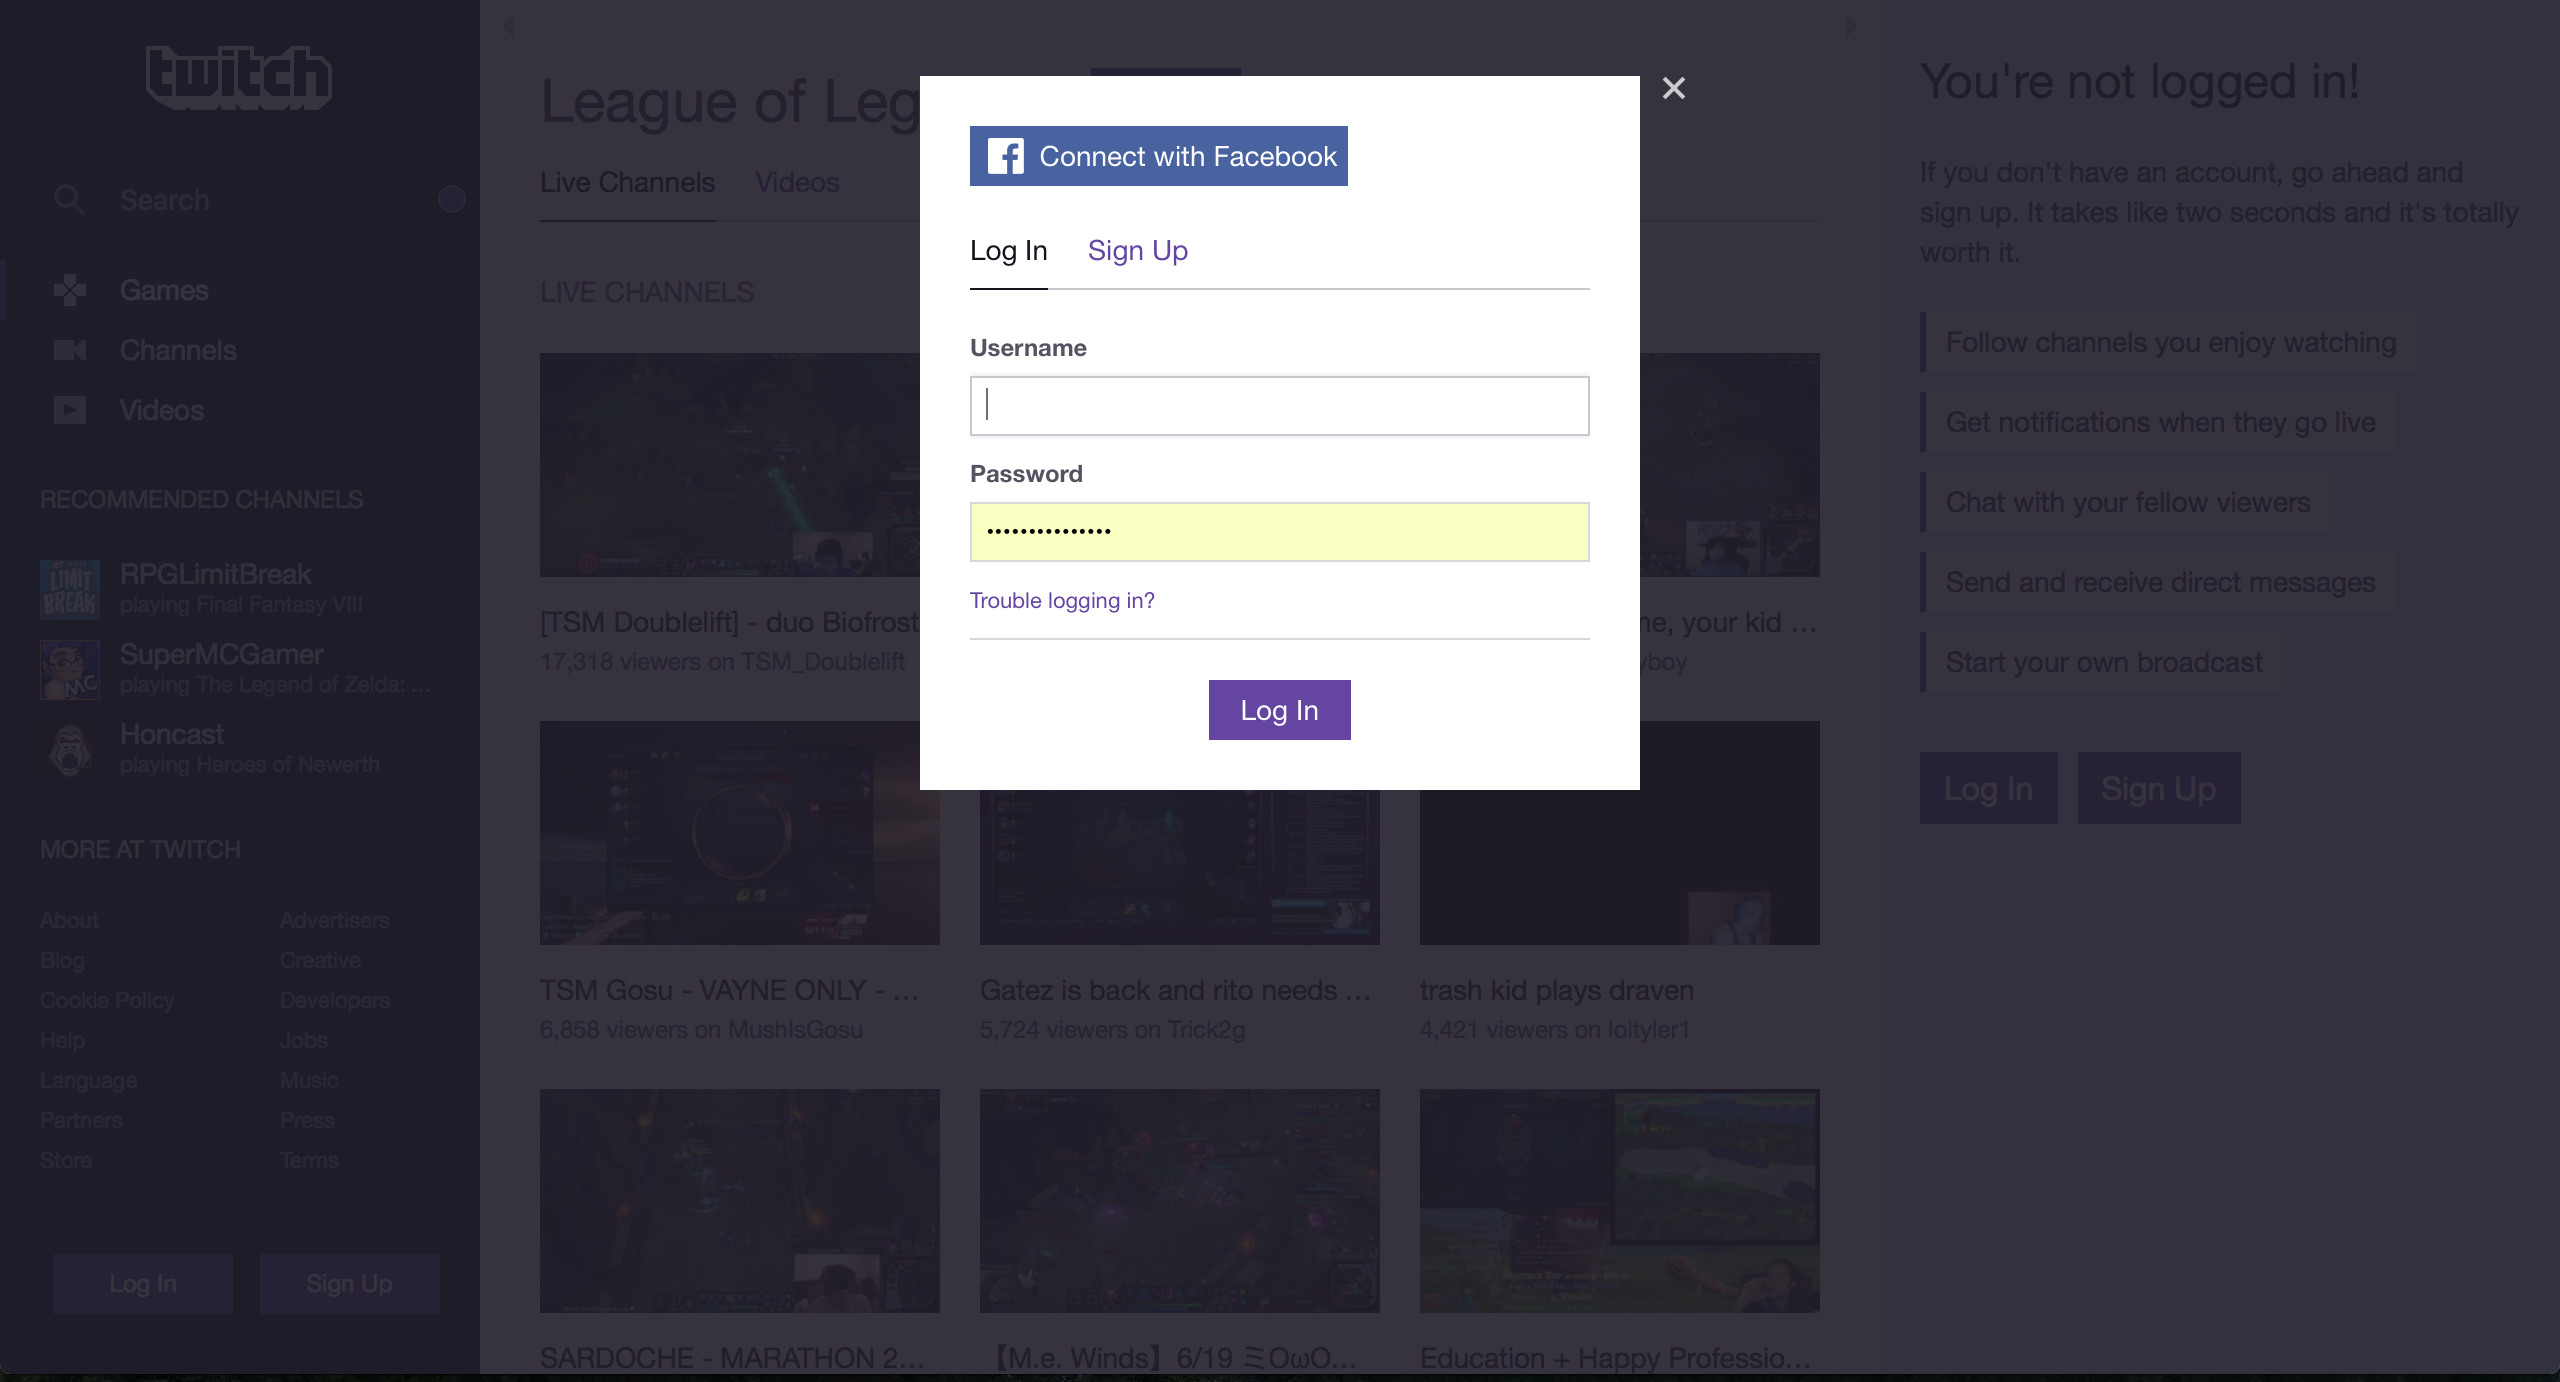
\includegraphics[scale=0.3]{img/auth.png}}
  \caption{Страница авторизации}
  \label{third}
\end{figure}

\begin{figure}[h!]
  \centering
  % Рамка только для изображений с белым фоном
  \fbox{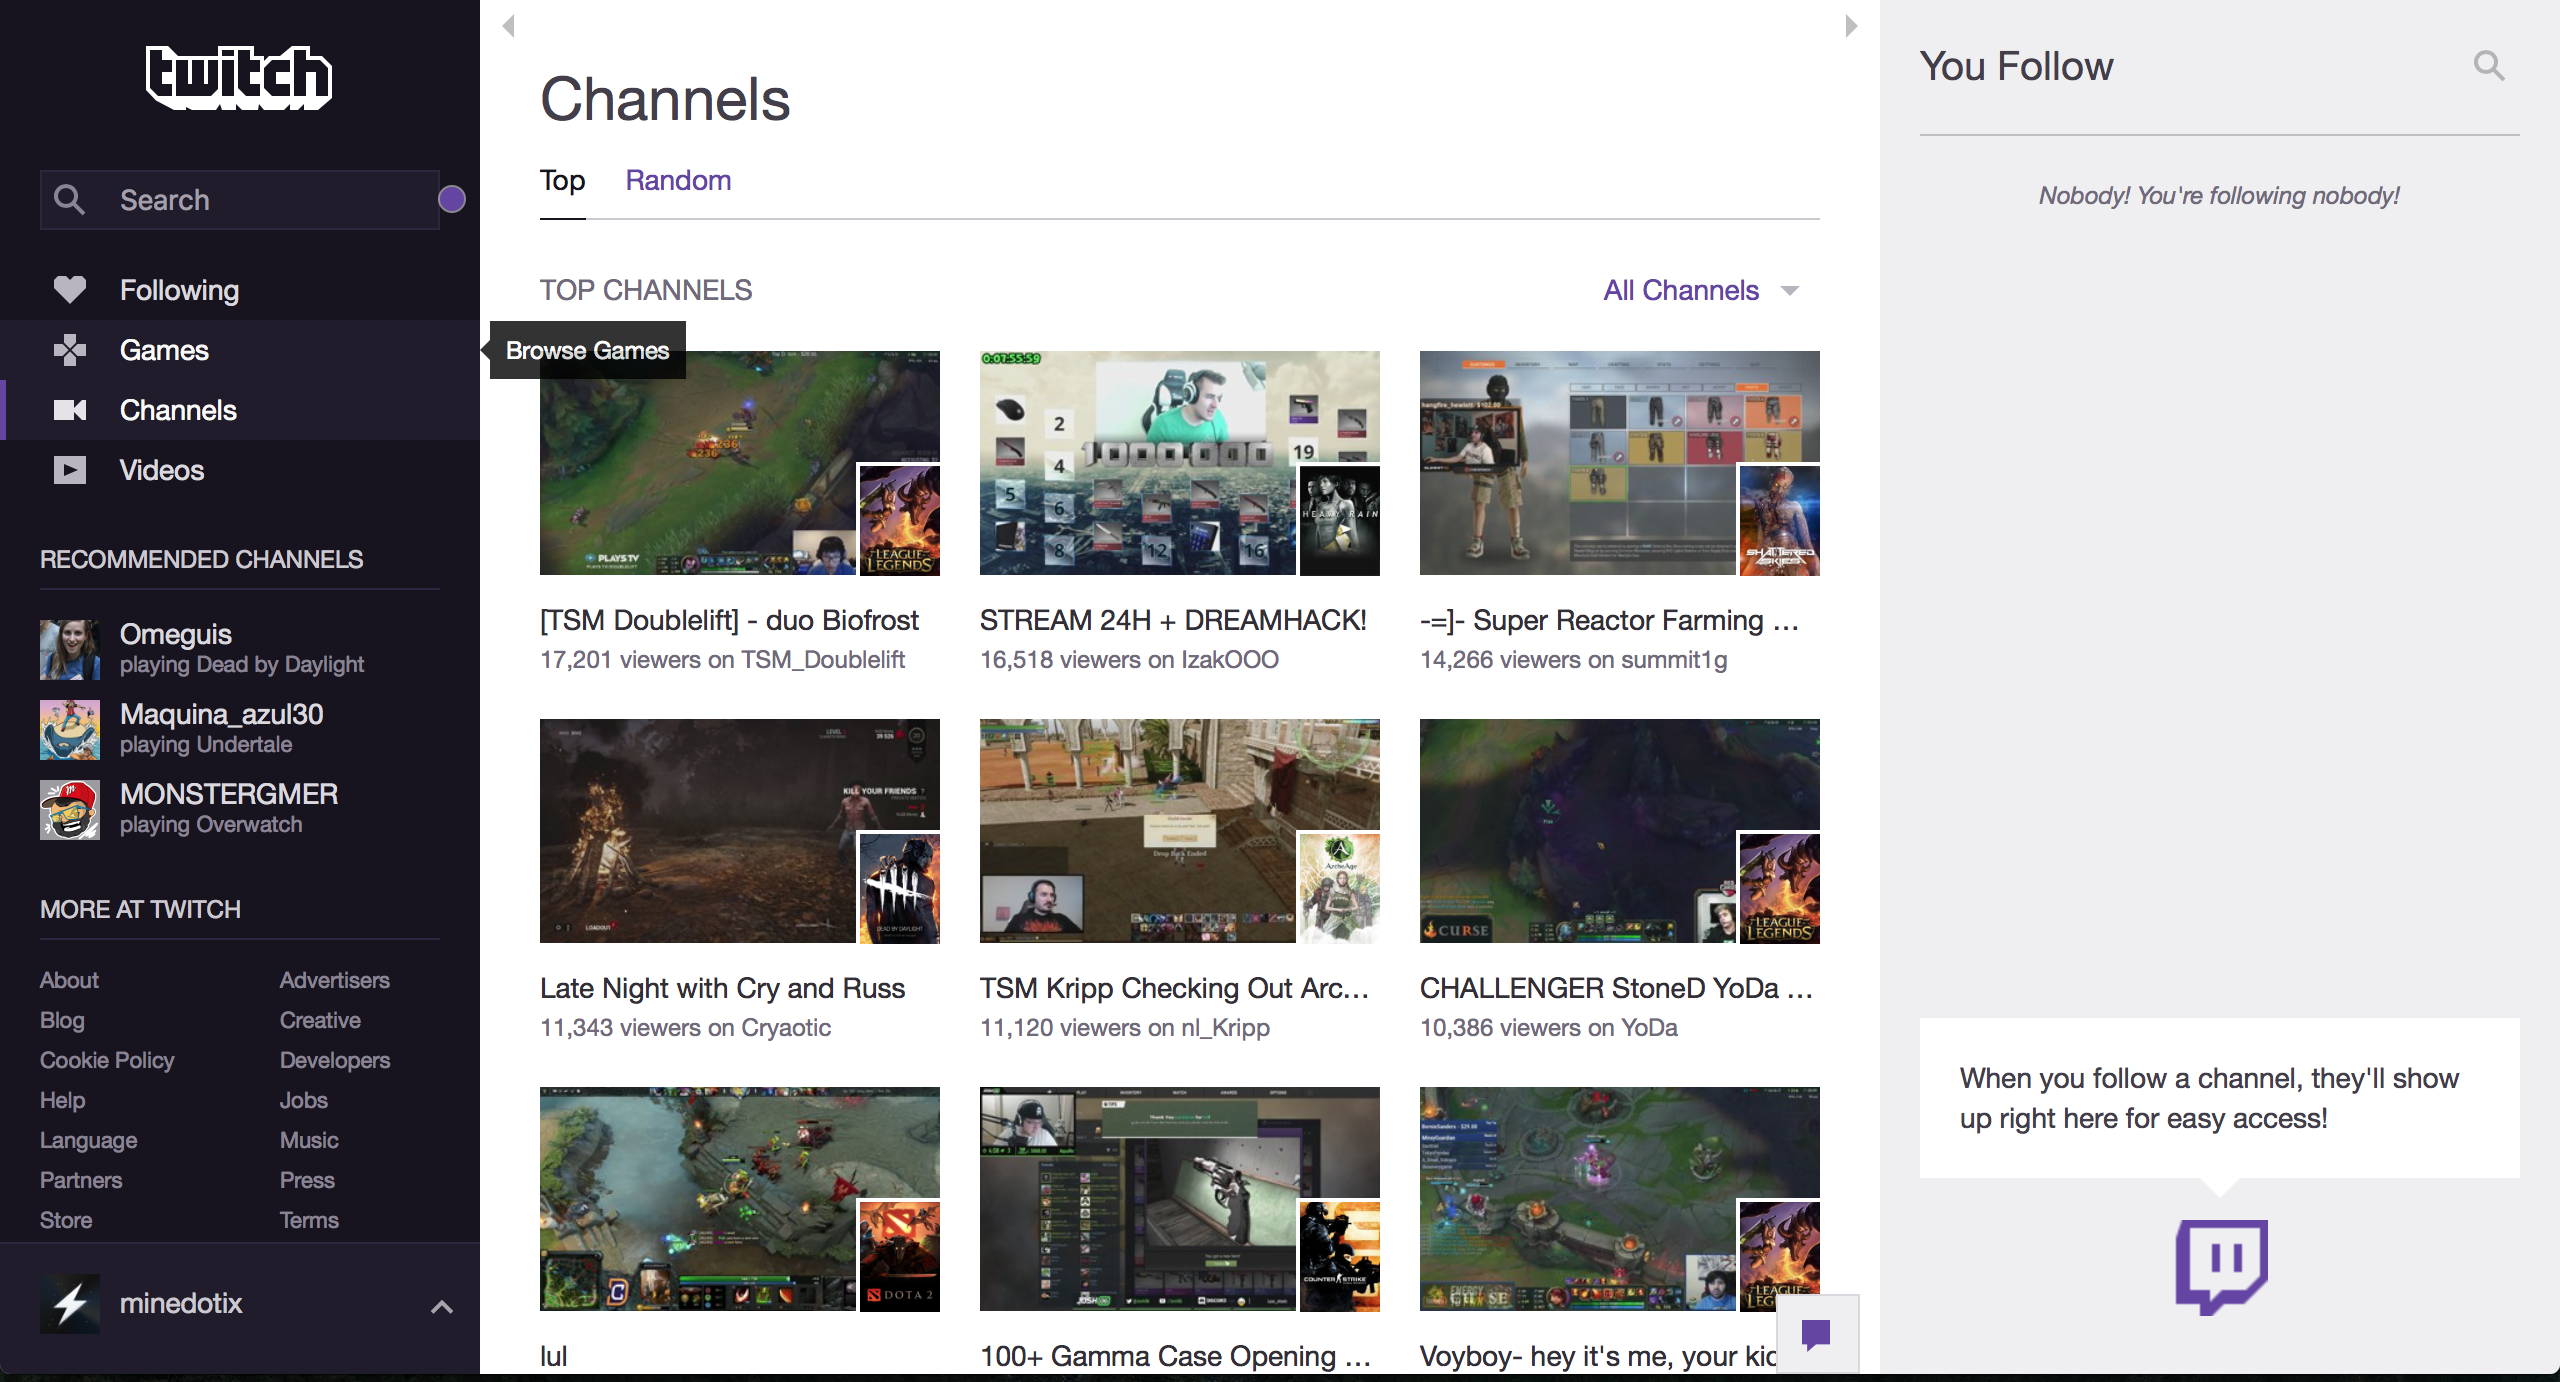
\includegraphics[scale=0.3]{img/catalog.png}}
  \caption{Каталог каналов}
  \label{third}
\end{figure}

\begin{figure}[h!]
  \centering
  % Рамка только для изображений с белым фоном
  \fbox{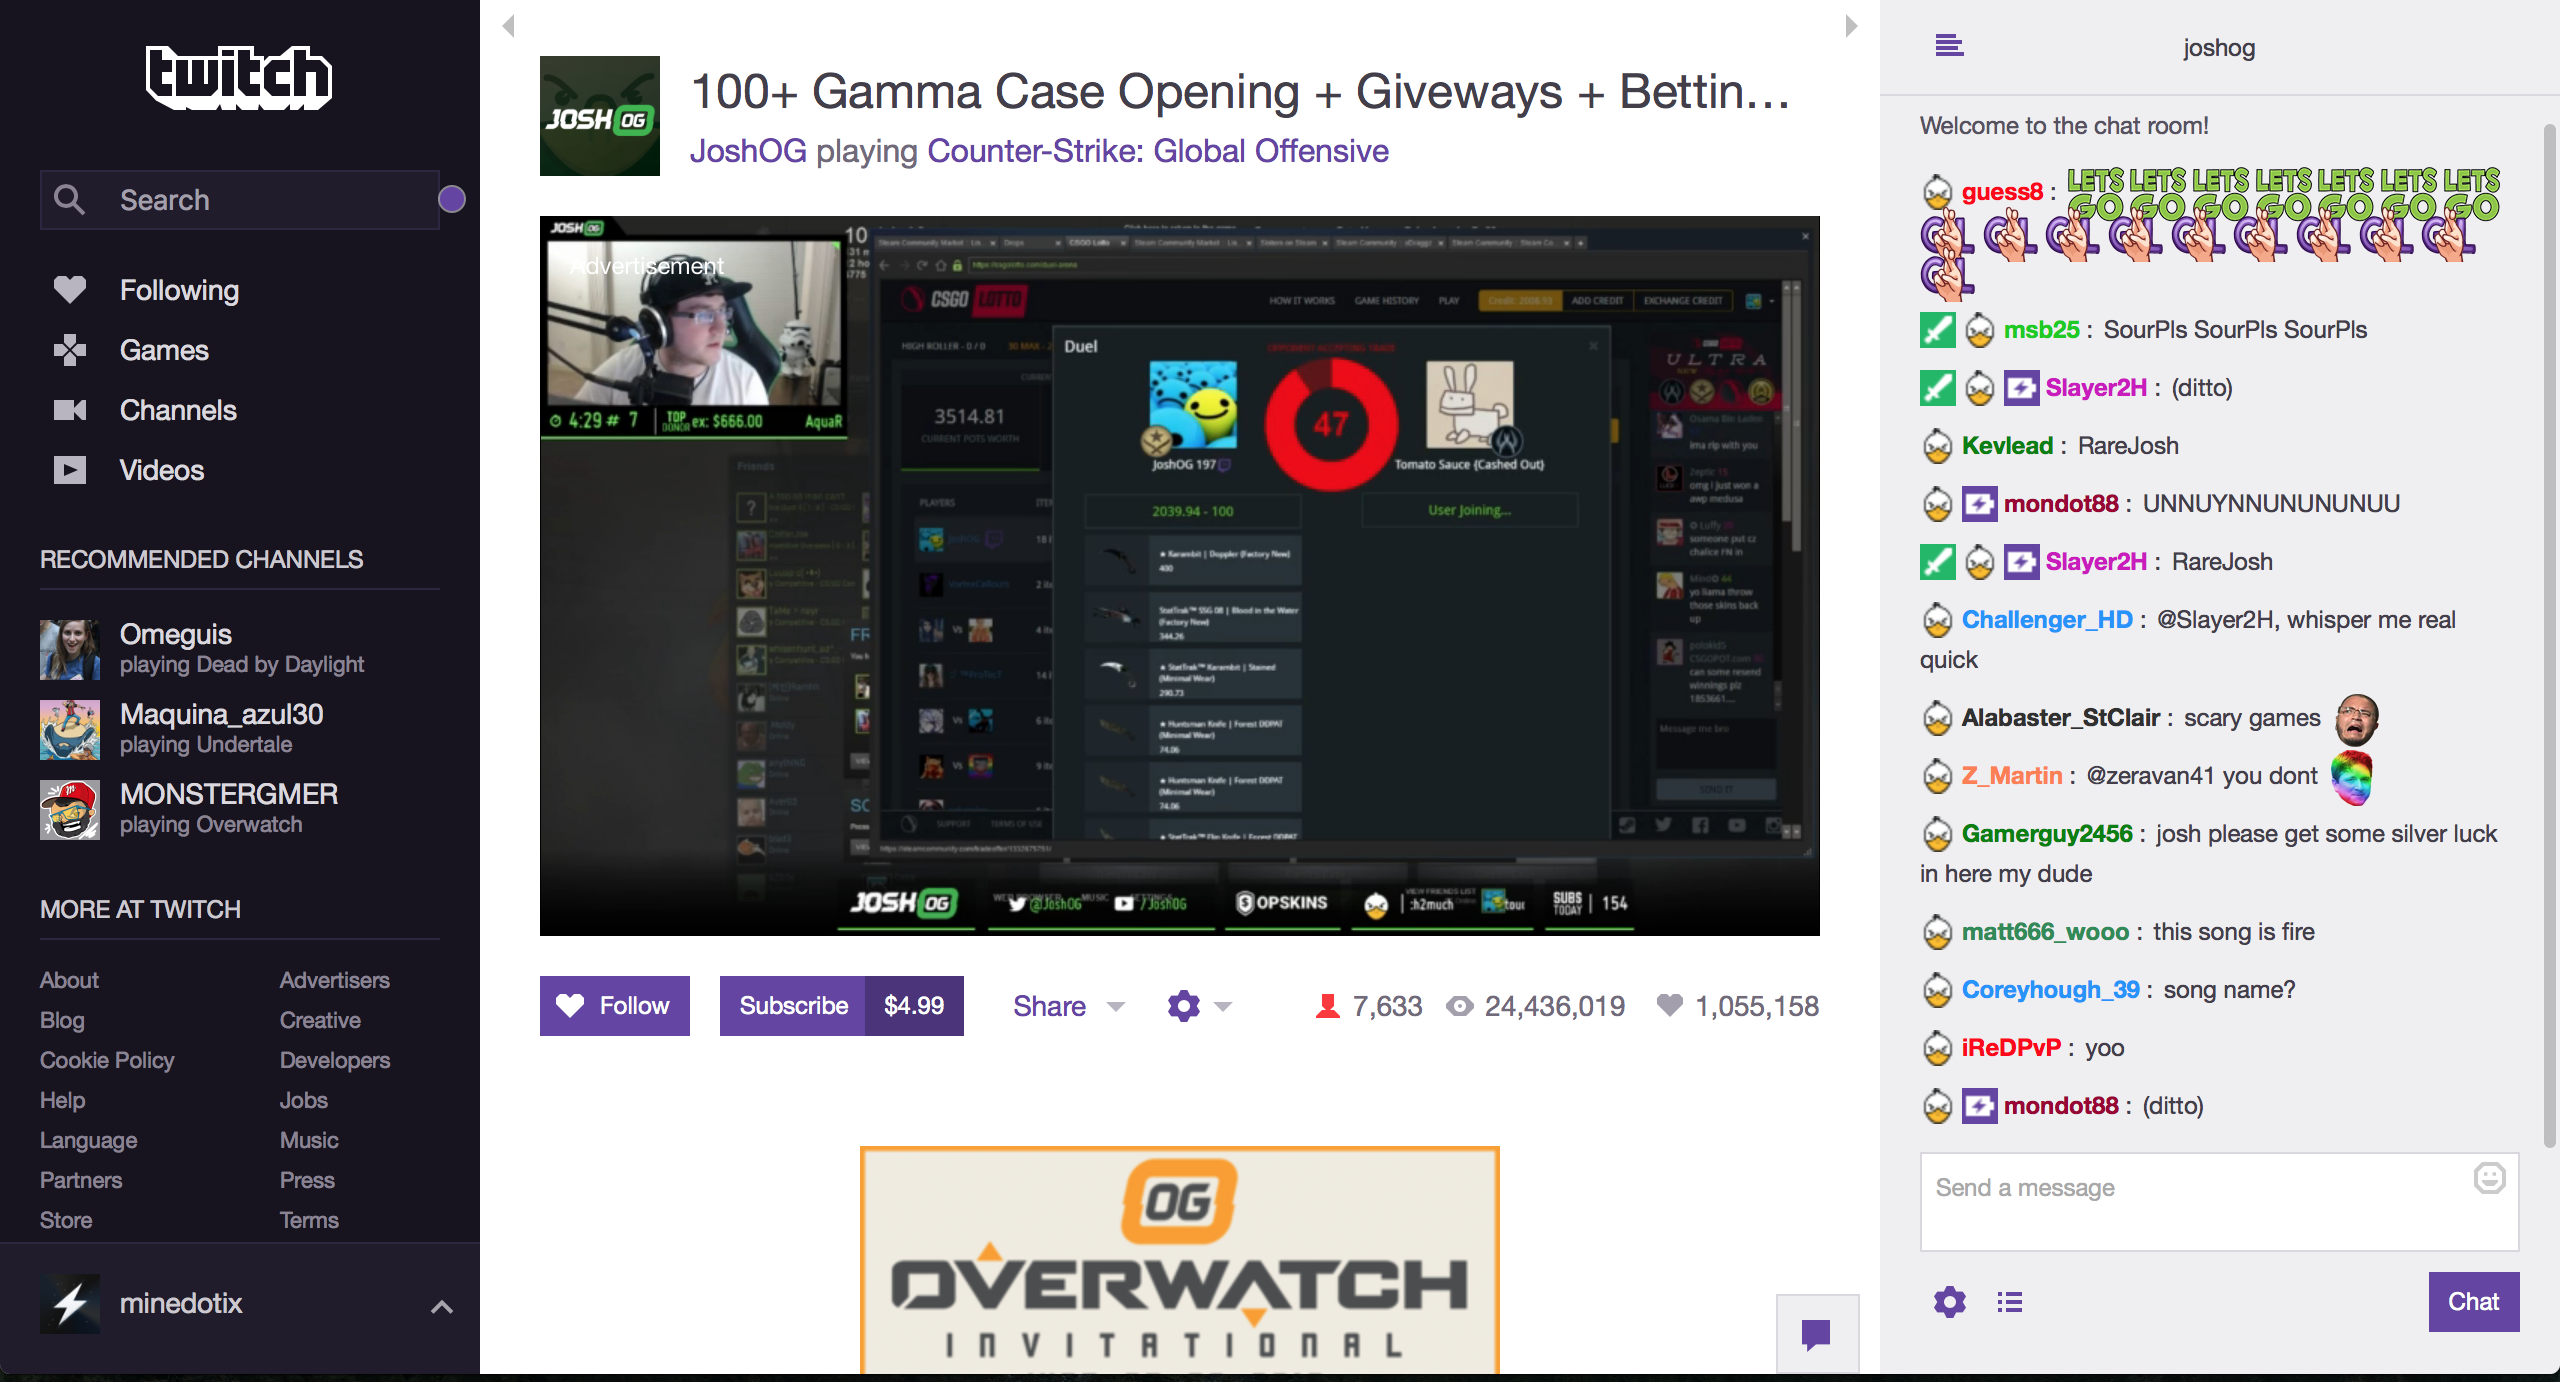
\includegraphics[scale=0.3]{img/channel.png}}
  \caption{Просмотр канала}
  \label{third}
\end{figure}

\section{Выбор технологии}
\subsection{Сервер}
Play Framework + Scala + Akka
\subsection{Клиент}
Backbone.js + React.js
\end{document}